\section{Модель процессов}

Описание модели процессов предметной области было выполнено в нотации UML.
~\cite{uml_rambo,uml_rosenberg} <<Лицевой>> диаграммой процессов является диаграмма
вариантов использования (рисунок~\ref{ris:3.2.1}).

\begin{figure}[h!]
\center{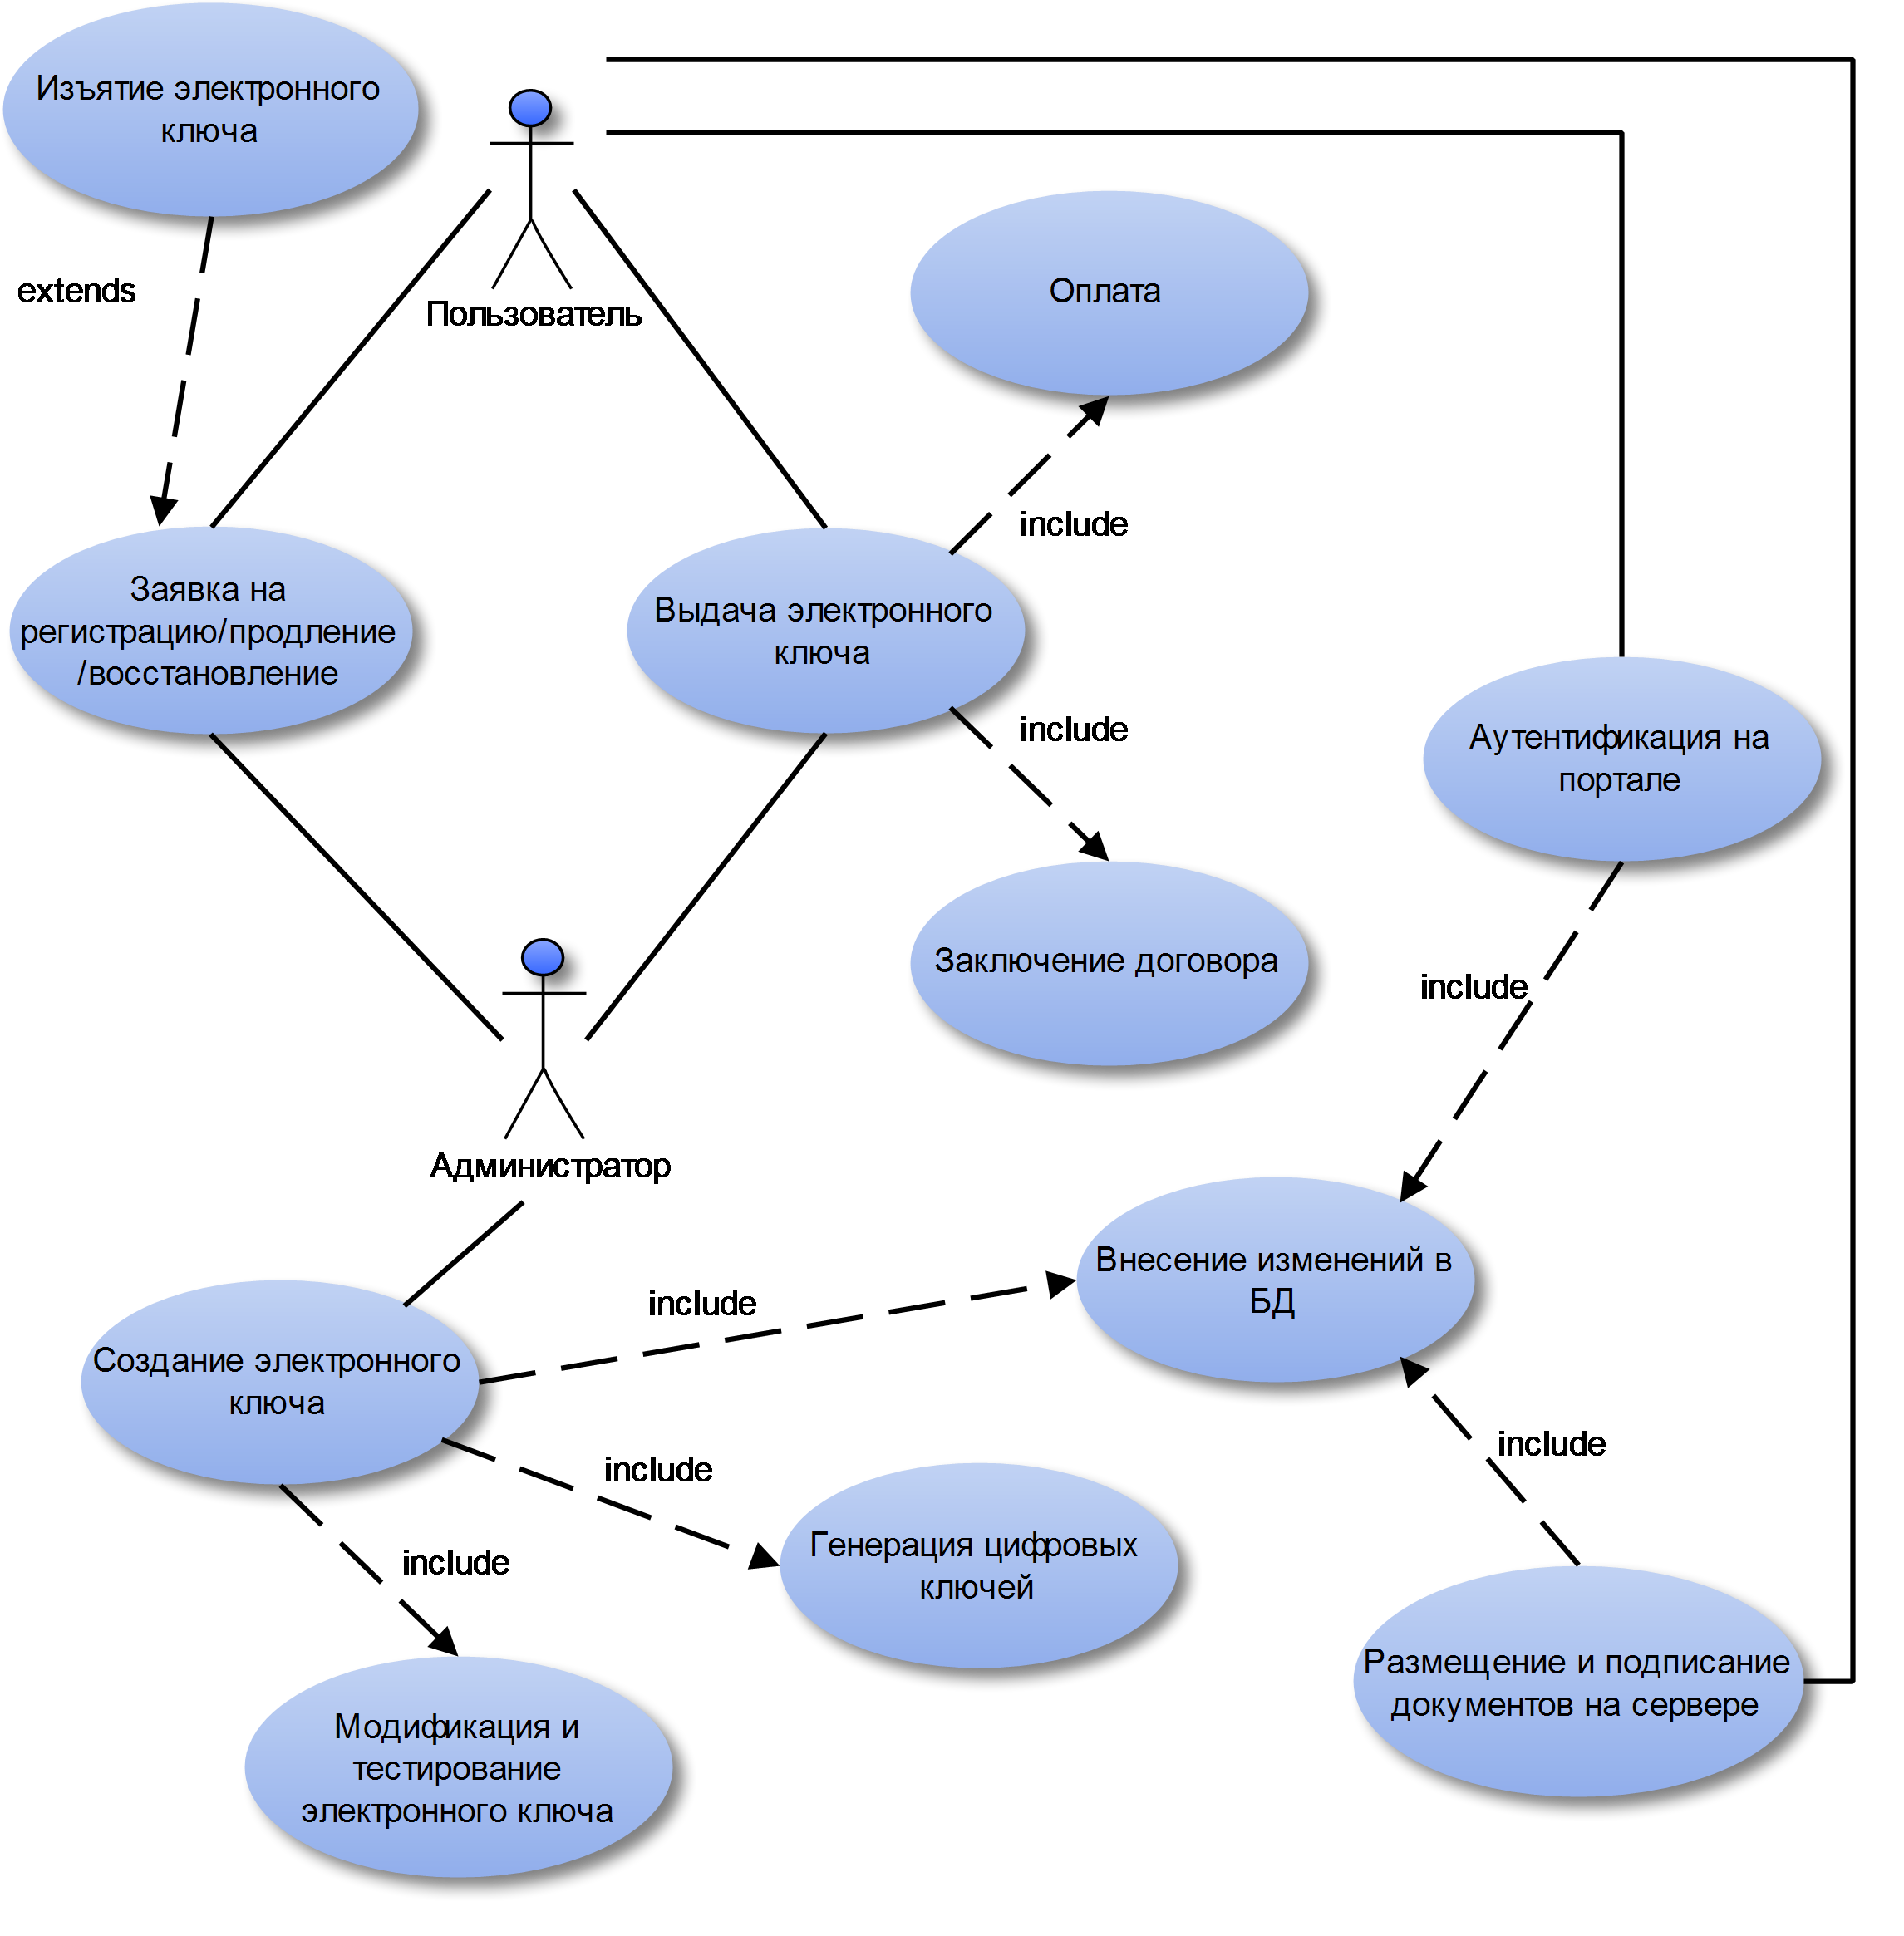
\includegraphics[width=1\linewidth]{3-2-1}}
\caption{Диаграмма вариантов использования}
\label{ris:3.2.1}
\end{figure} 

\begin{figure}[h!]
\center{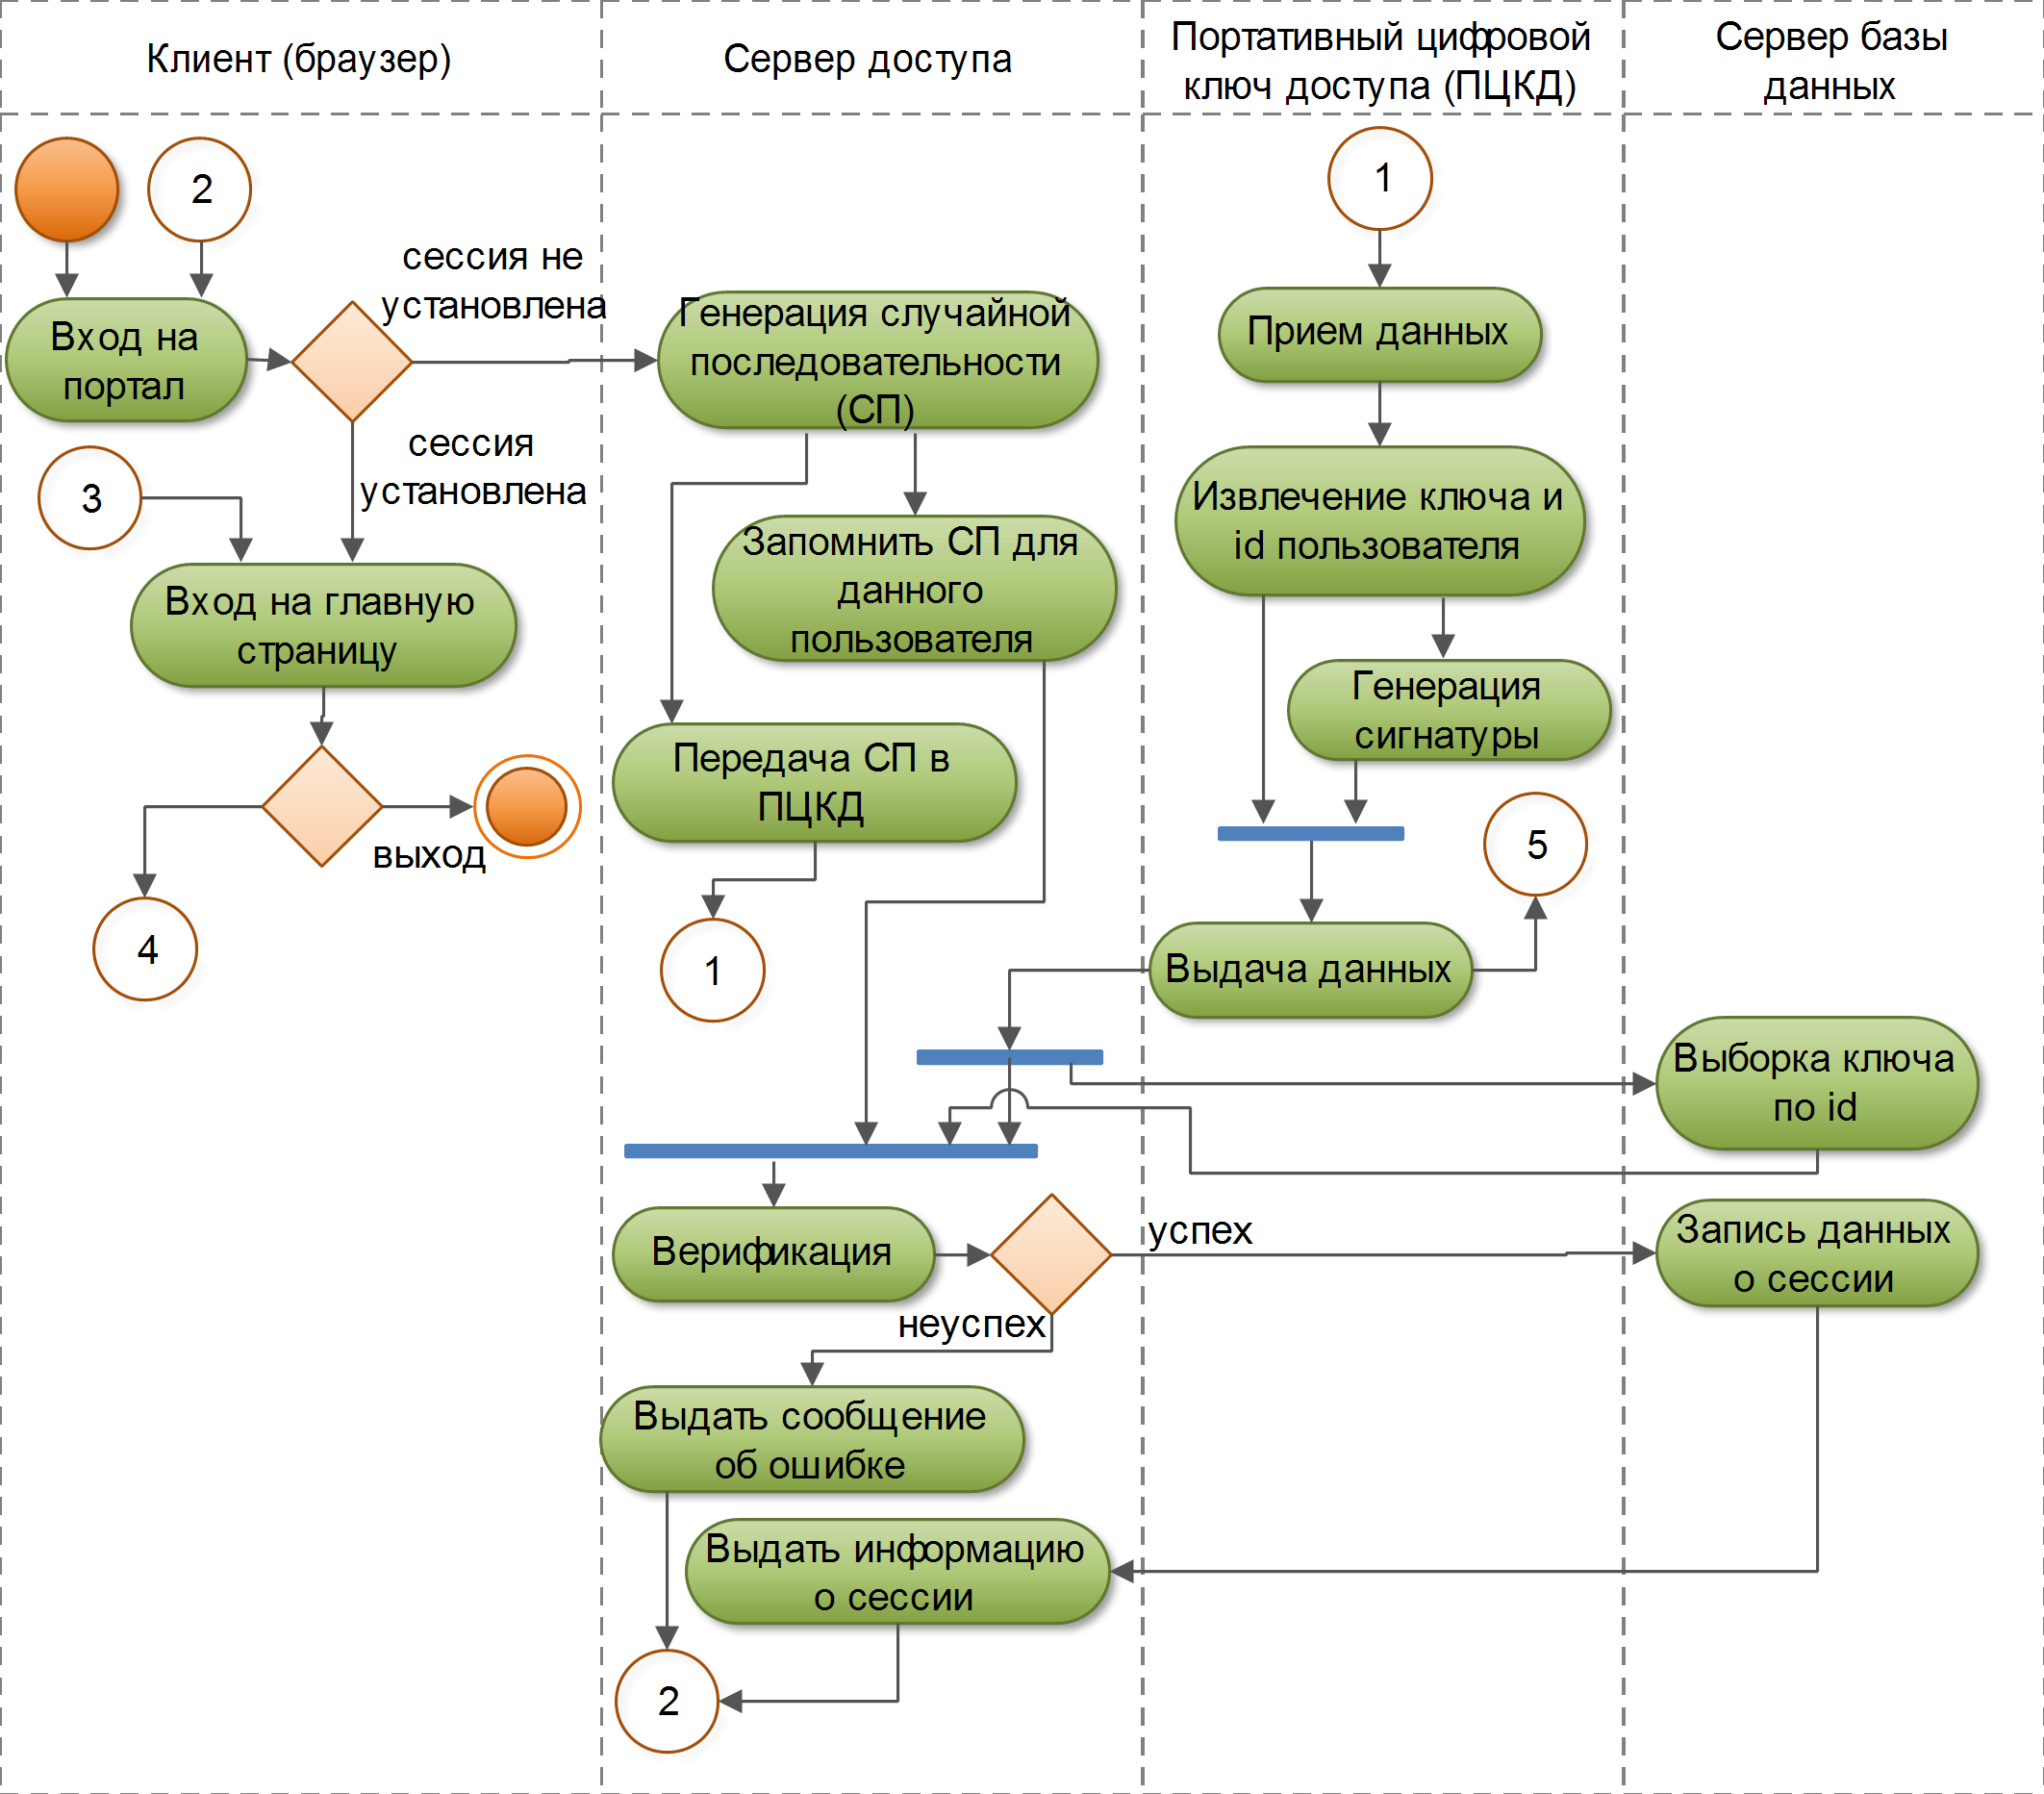
\includegraphics[width=1\linewidth]{3-2-2}}
\caption{Диаграмма активности (часть 1)}
\label{ris:3.2.2}
\end{figure} 

\begin{figure}[pH]
\center{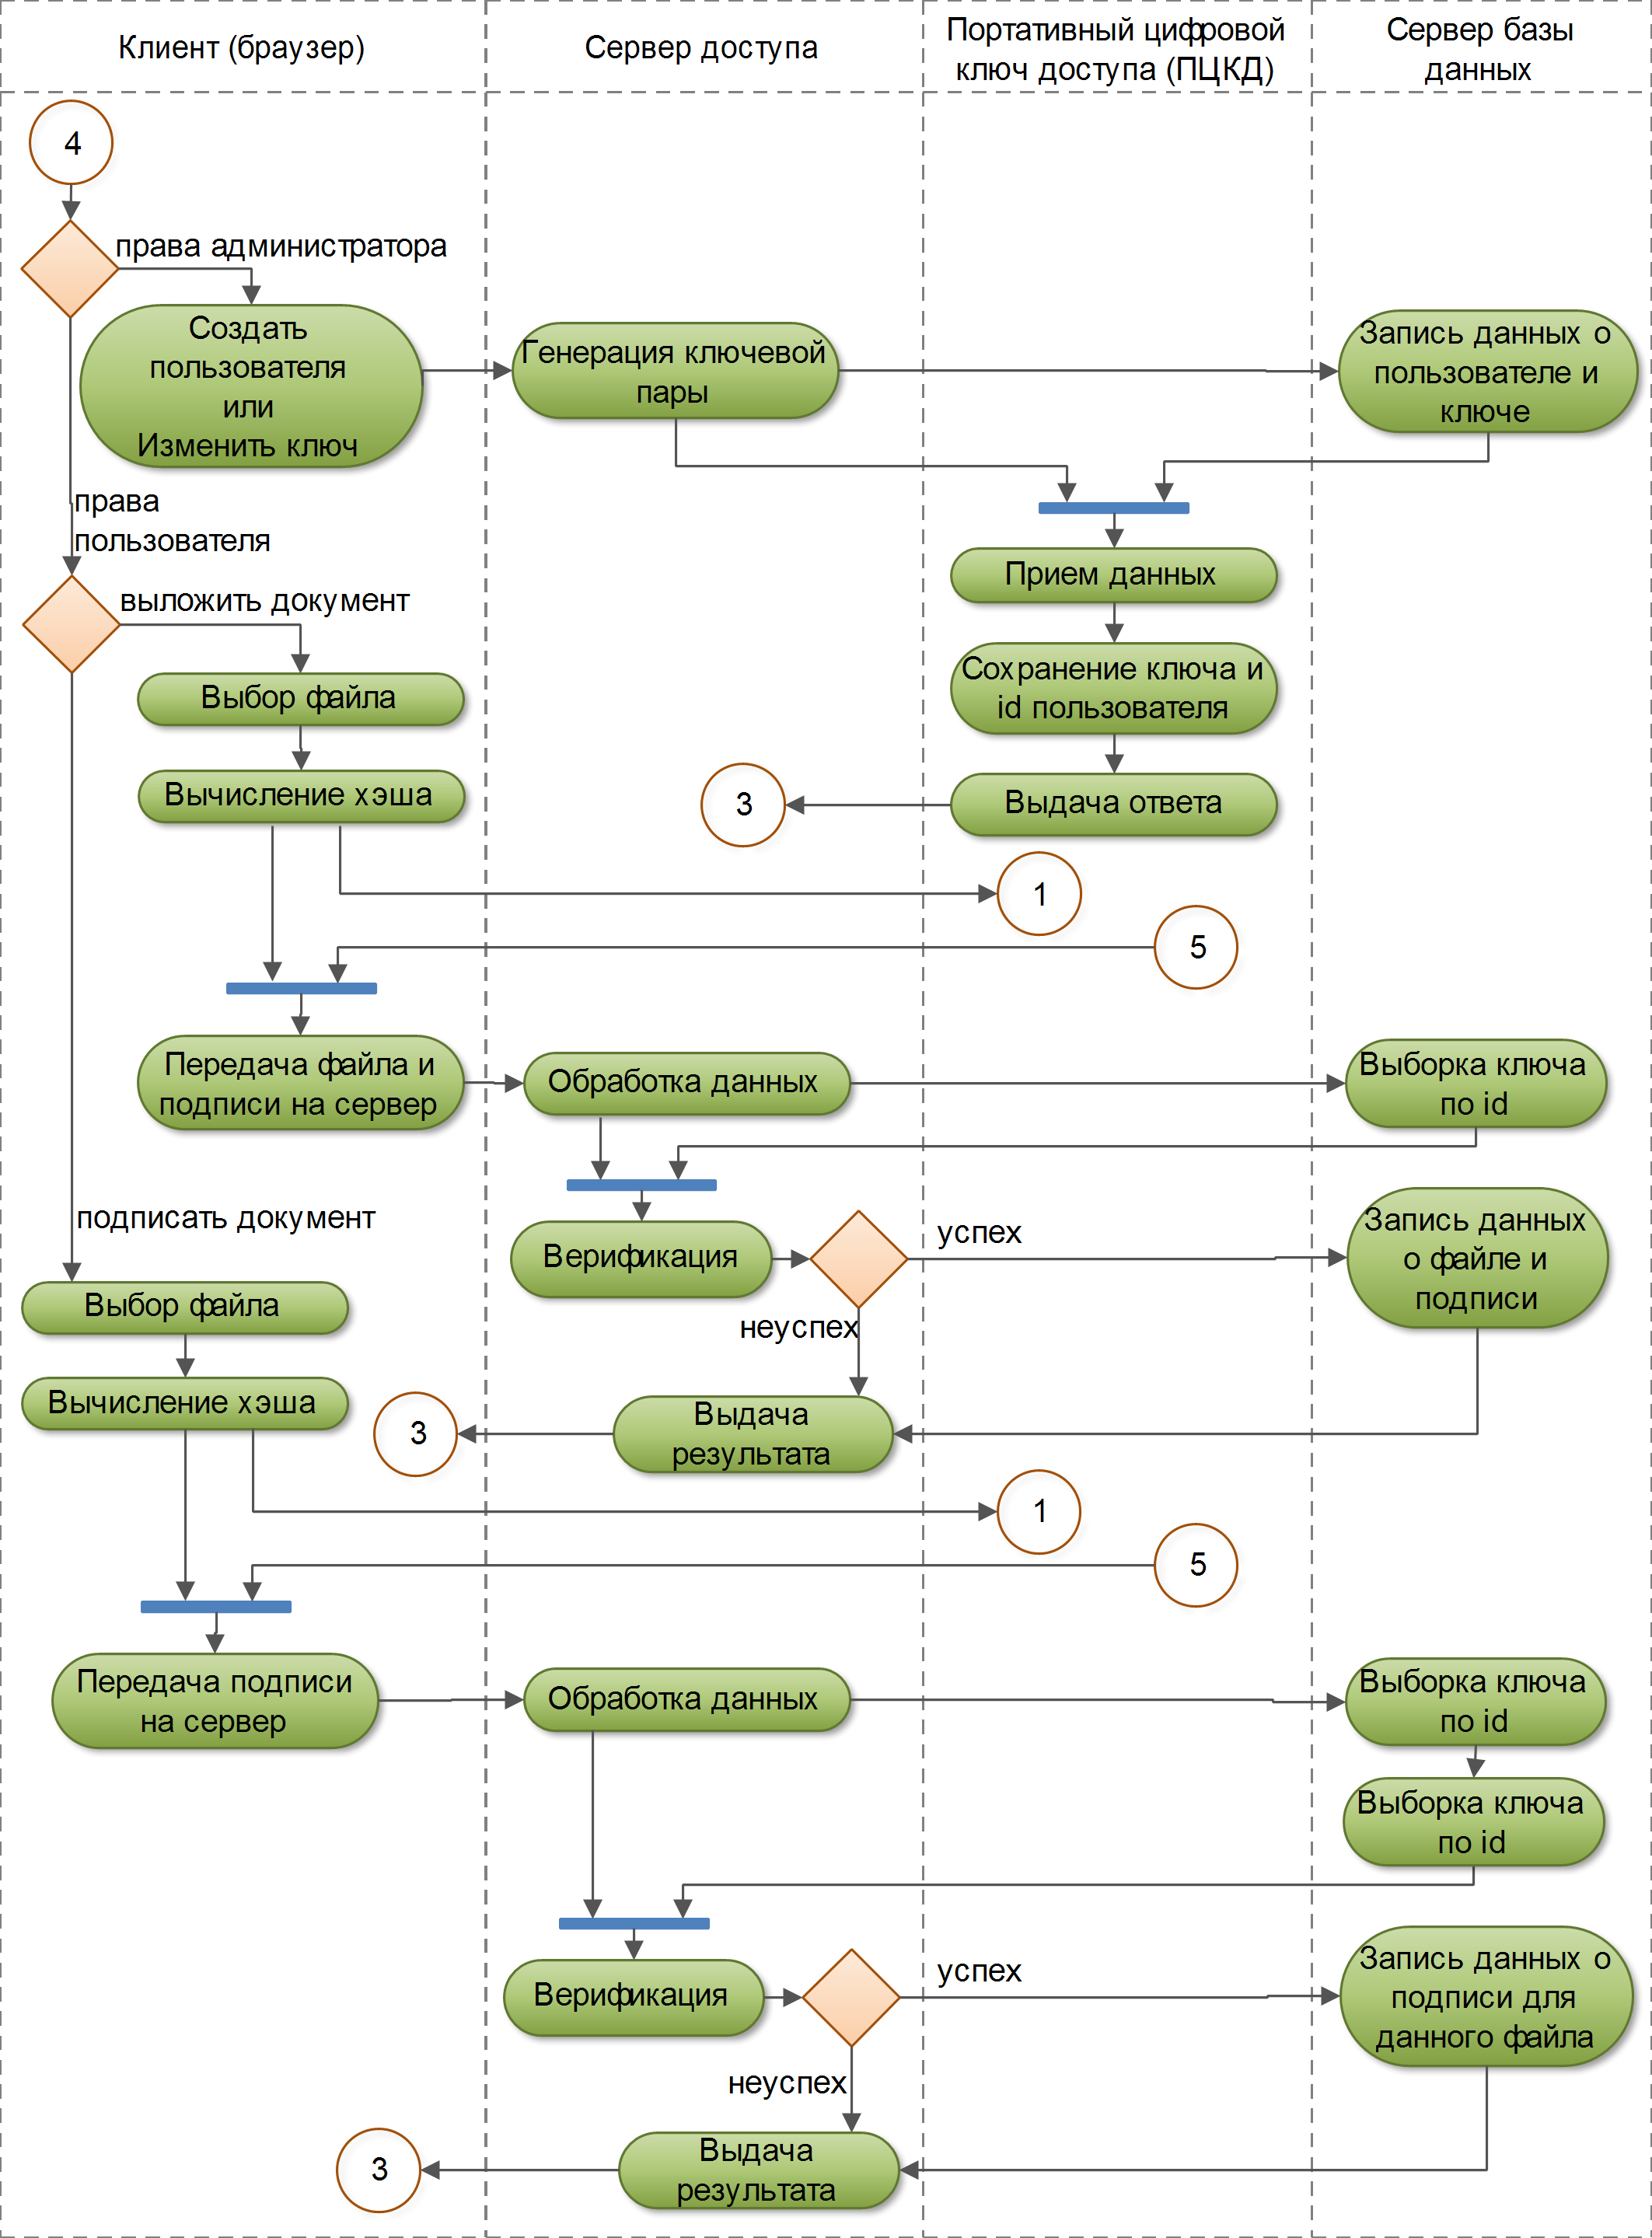
\includegraphics[width=1\linewidth]{3-2-3}}
\caption{Диаграмма активности (часть 2)}
\label{ris:3.2.3}
\end{figure} 

Основными функциональными действиями пользователя являются: аутентификация на
портале и размещение и подписание документов на сервере. Данные операции в
обязательном порядке вносят записи в базу данных.

Для осуществления данных функций, пользователю необходимо обладать портативным
цифровым ключем доступа (электронным ключем), который можно получить при
взаимодействии с администратором сервиса. Для этого необходимо подать заявку на
регистрацию/продление/восстановление электронного ключа, после чего ключ будет
выдан пользователю. В случае продления ключа старый ключ изымается у
пользователя. Выдача электронного ключа сопровождается заключением договора с
пользователем и оплатой.

Создание нового электронного ключа включает генерацию цифровых ключей, внесение
соответствующей информации в базу данных, а так же модификацию и тестирование
портативного цифрового устройства доступа.

Детализация диаграммы вариантов использования получила свое продолжение в виде
диаграммы активности (рисунок~\ref{ris:3.2.2} и рисунок~\ref{ris:3.2.3}).
Данная диаграмма наиболее точно и полно детализирует рассматриваемый процесс. 

\begin{figure}[h!]
\center{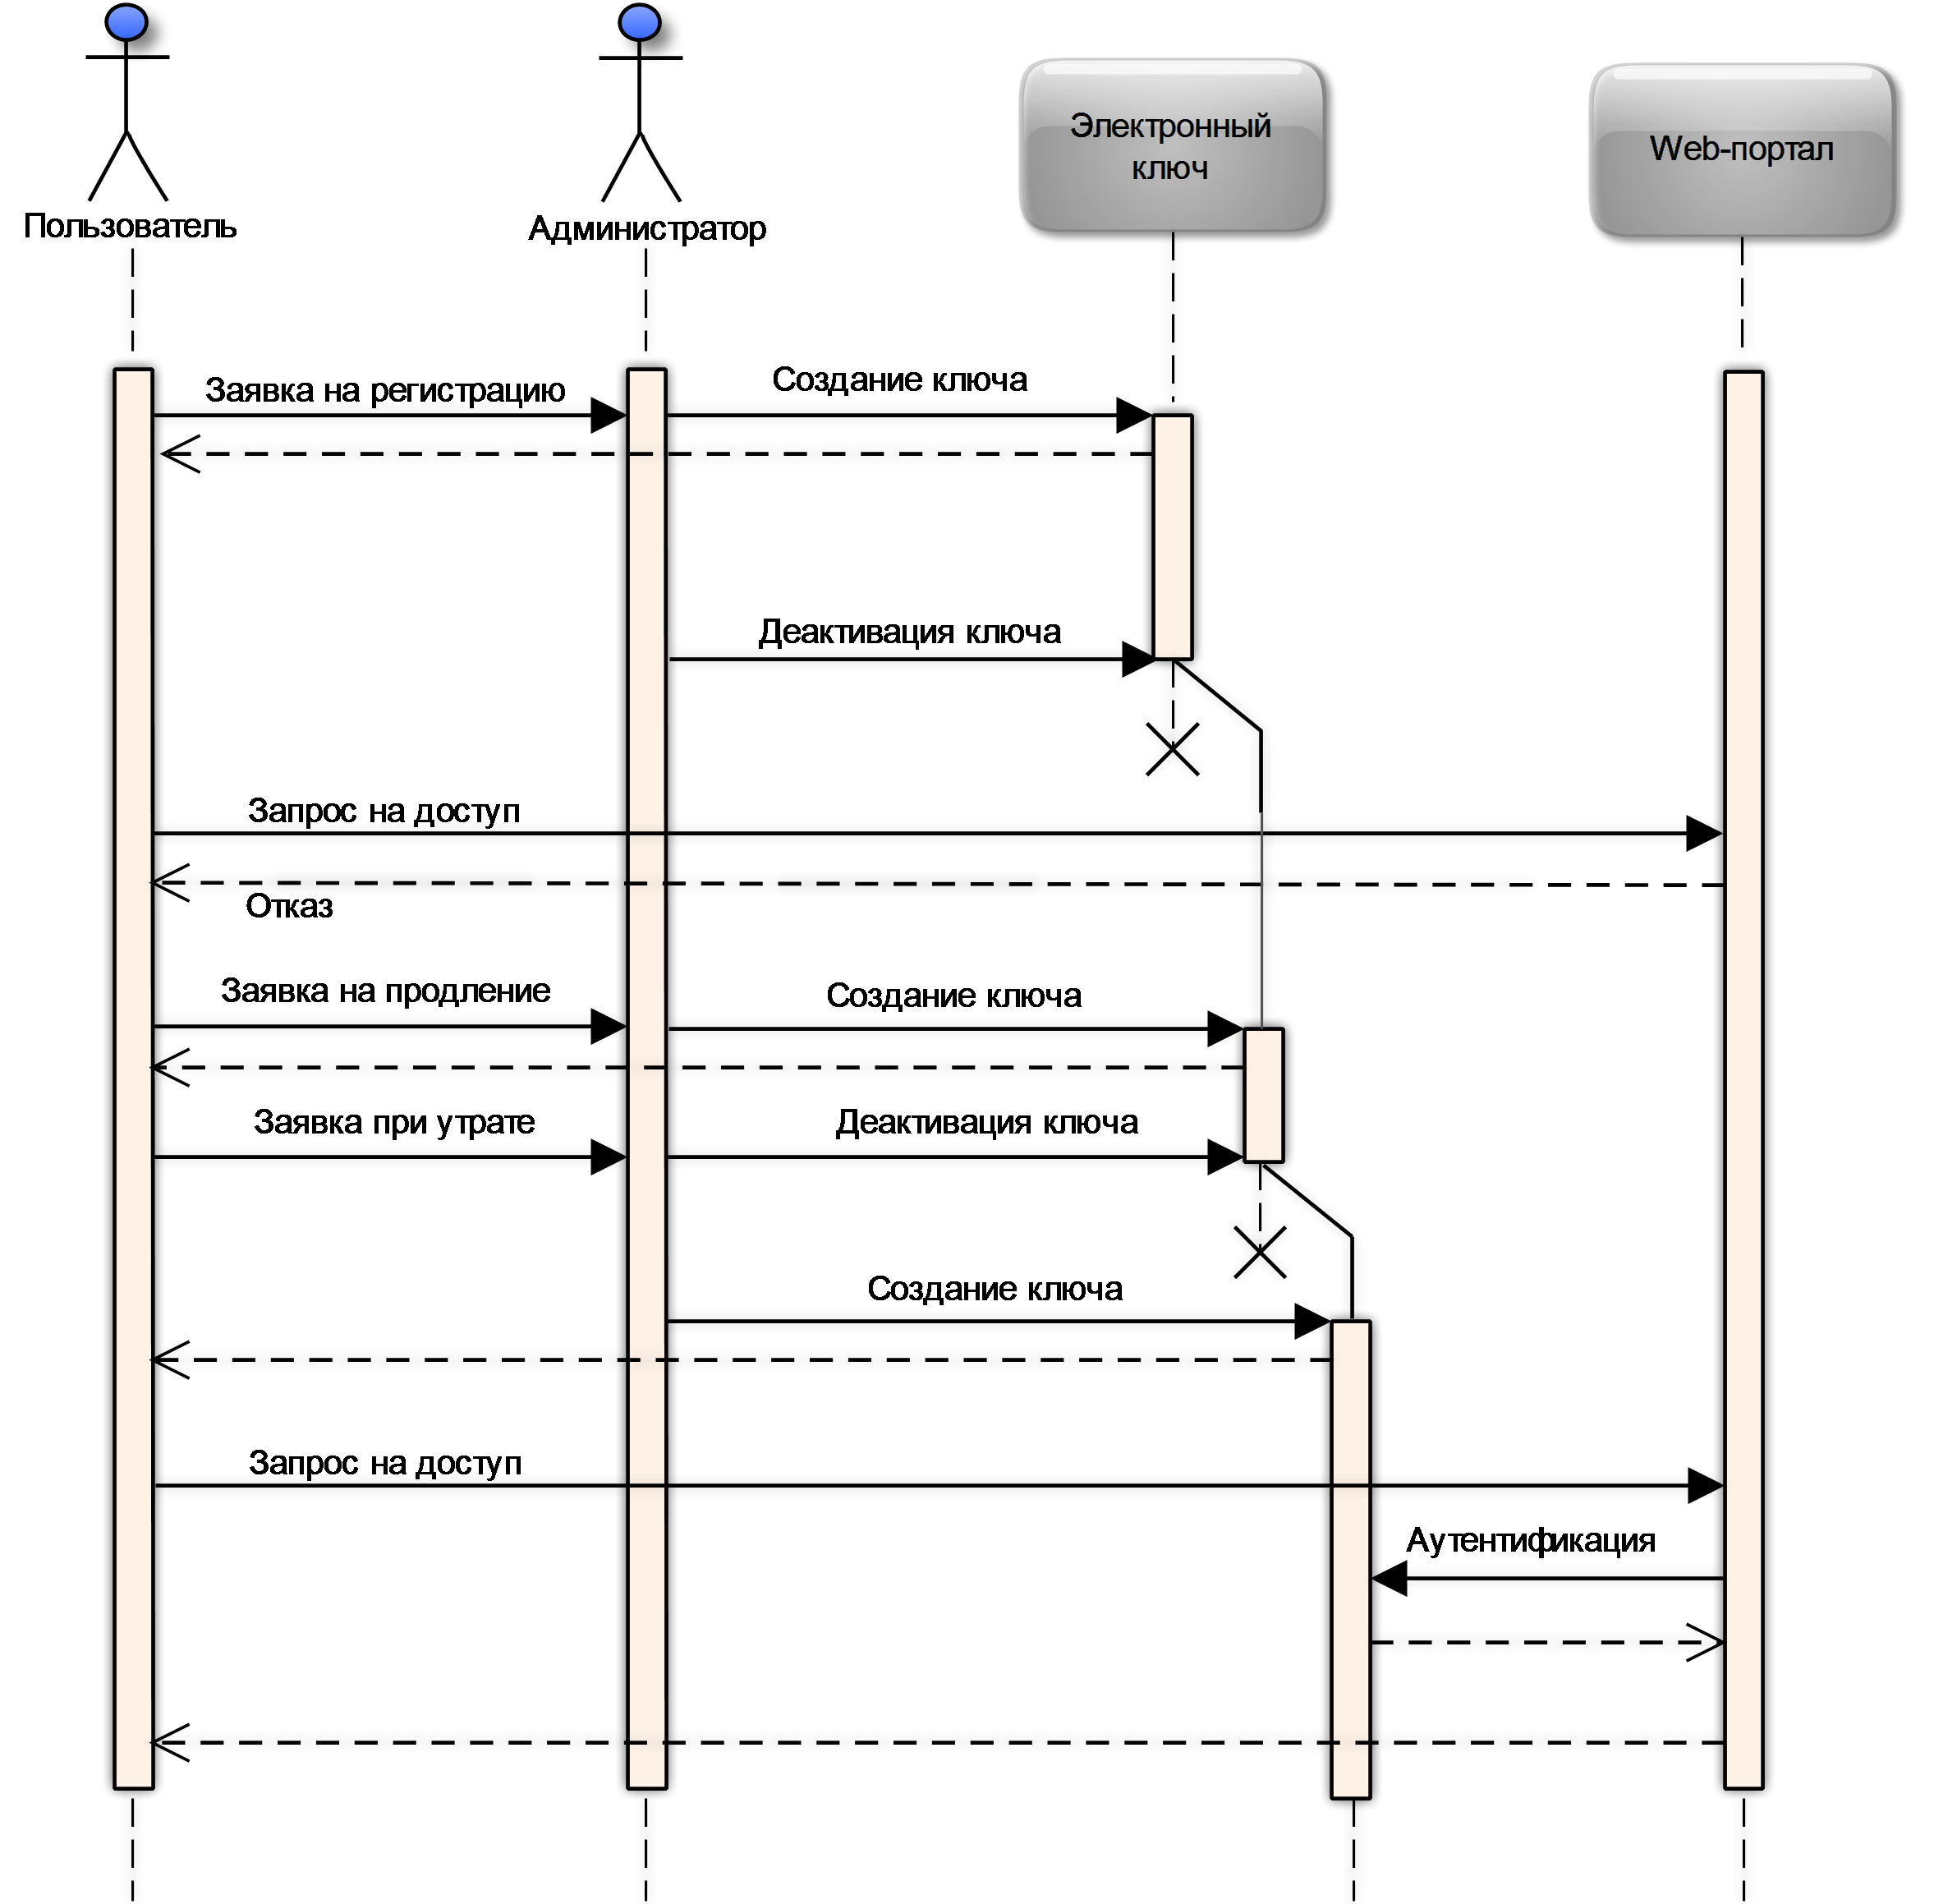
\includegraphics[width=1\linewidth]{3-2-4}}
\caption{Диаграмма взаимодействия}
\label{ris:3.2.4}
\end{figure} 

Диаграмма взаимодействия, фрагмент которой изображен на рисунке
~\ref{ris:3.2.4}, отображает линию жизни электронного ключа, а также действия
акторов в различных ситауциях.

Если пользователь еще не зарегистрирован в системе, то необходимо подать заявку
на регистрацию, после чего администратор создаст ключ, который будет передан
пользователю. По истечении установленного срока службы ключа произойдет
деактивация ключа и пользователь не сможет войти на портал с утратившим силу
ключом. В этом случае пользователь подает заявку на продление срока службы
ключа. При этом происходит изъятие устаревшего ключа, создание нового и выдача
обратно пользователю.

В случае утраты электронного ключа необходимо незамедлительно подать заявку
администратору, после чего ключ будет деактивирован и тут же создан новый. После
чего пользователь может получать доступ на портал в обычном режиме.